\chapter{Related work}
\label{chap:rel_work}

\section{Linked Data}

This section explores the related work in linked traversal-based query processing, focusing on the fundamental concepts and technologies that form the backbone of the Linked Data ecosystem. The discussion begins with a concise definition of Linked Data and an examination of the principles put forth by Tim Berners-Lee, emphasizing the importance of unique URIs, dereferencing, and data linking. Subsequently, the Resource Description Framework (RDF) is explored as the foundational data model for representing knowledge in Linked Data format. RDF Schema (RDFS) and Web Ontology Language (OWL) are then introduced to extend the capabilities of RDF by allowing the definition of ontologies and richer semantics. Moving forward, the attention shifts to JavaScript Object Notation for Linked Data (JSON-LD) as a popular format for representing Linked Data in JSON, with a focus on its incorporation of Linked Data principles within JSON documents. The discussion continues with an exploration of SPARQL and query interfaces, encompassing the syntax, capabilities, and different interfaces for efficient access and retrieval of Linked Data. Finally, the section concludes by examining the challenges and advantages associated with Linked Data, emphasizing the importance of addressing data quality, scalability, integration, and the potential benefits of improved interoperability and knowledge graph creation. This comprehensive exploration of related work provides a solid foundation for the subsequent discussions on linked traversal-based query processing.

\subsection{Introduction and Principles}

To better understand the origins of the idea behind Linked Data, it is important to examine the origins of the World Wide Web. For example, its first, but still rather primitive, underlying technology was introduced in 1989 at CERN. Tim Berners-Lee was the man responsible for its development. By using HyperText Markup Language (HTML), it enabled scientists, and later the rest of the world, to publish documents that could contain links to other documents. This helped create a mesh of documents and information. However, since these documents in fact contained nothing more than raw data dumps and links between documents represented simply an indication of how to reach the document, these documents and their relationships lacked semantics. Figure~\ref{fig:no_linked_data} illustrates what a web of documents without unambiguous indications of what their contents and the links between them represent, might look like. It is necessary to note here that the used icons are not the contents of their respective documents, but only a representation of their contents. Nevertheless, in themselves, they prove the weakness of such web as much as when the effective content of the documents had been represented. After all, just from the raw content of documents and their mutual links, a person cannot clearly infer exactly what their constellation represents, let alone a computer. From that deficiency, therefore, emerged the idea of Linked Data. \citep{jacksi2019development} \citep{bizer2011linked}

\begin{figure}[htbp]
    \centering
	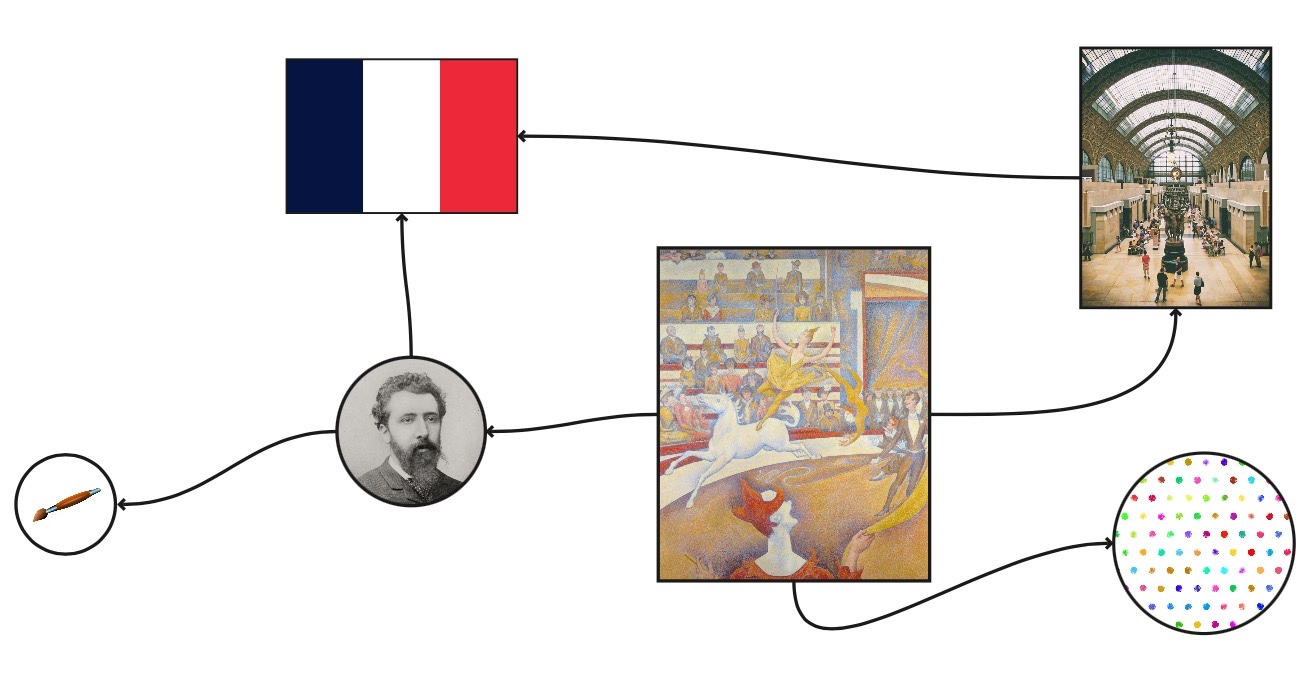
\includegraphics[width=\textwidth]{images/no_linked_data.jpg}
    \captionsetup{justification=centering}
	\caption{Representation of a web of documents without unambiguous indications of what the documents and the links between them represent}
	\label{fig:no_linked_data}
\end{figure}

Simply put, data coming from different sources can be labeled as Linked Data as soon as they are linked by typed links. In other words, links are no longer just an indication of how to reach another document. Indeed, within the Linked Data story, they also contain information about what exactly the link in question represents. Linked Data thereby ensures the meaning of data is explicitly defined, in turn rendering the data machine-readable. Figure~\ref{fig:linked_data} represents the same web of documents as Figure~\ref{fig:no_linked_data}, but this time in accordance with the idea of Linked Data. Indeed, the documents have been given an  unambiguous indication of what they represent, and their mutual semantics have also been clarified thanks to the labeling of their links. \citep{bizer2011linked}

\begin{figure}[htbp]
    \centering
	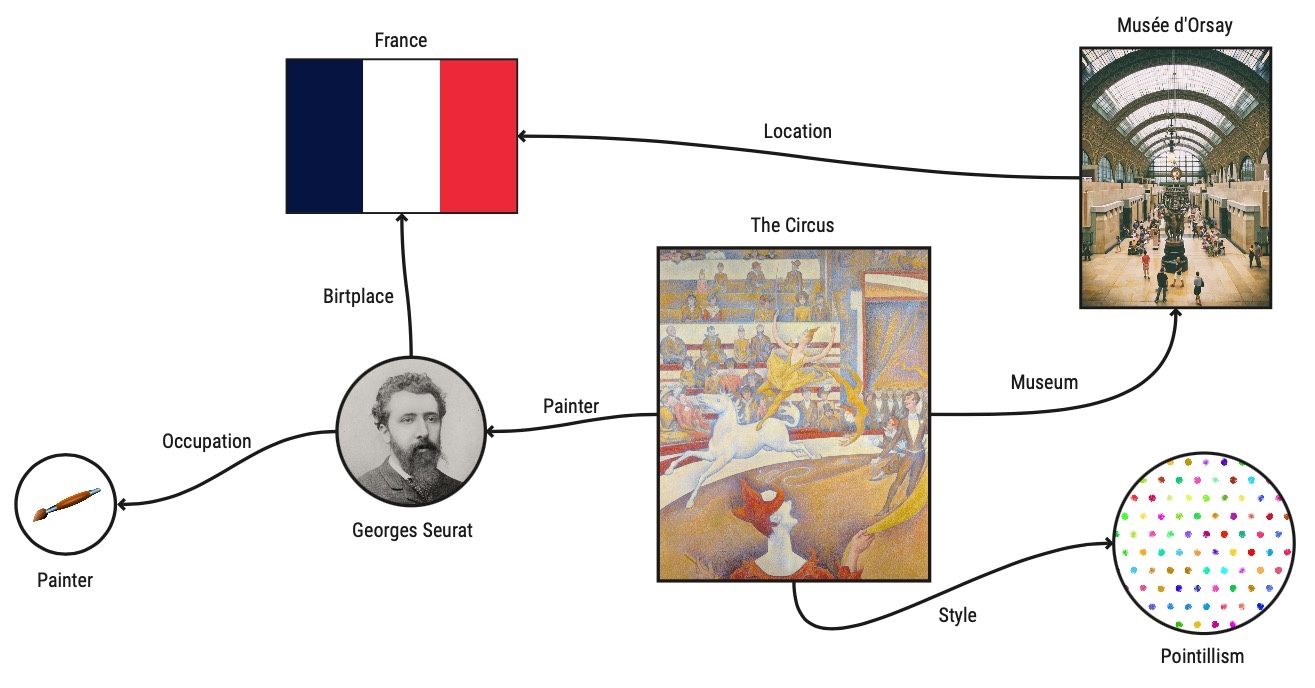
\includegraphics[width=\textwidth]{images/linked_data.jpg}
    \captionsetup{justification=centering}
	\caption{Representation of a web of documents composed according to the spirit of Linked Data}
	\label{fig:linked_data}
\end{figure}

Although several technologies exist to achieve the goals of Linked Data, the use of URIs is essential. After all, since URIs are unique, they can unambiguously reference a particular entity. Practically speaking, the URIs that appear in a Linked Data document can be dereferenced using the HTTP protocol in order to retrieve the underlying entities. For instance, \mintinline{text}{https://stad.gent/id/concept/530010539}, is a URI that can be dereferenced using the HTTP(S) protocol. By dereferencing URI after URI in this way, little by little a - what could be called - \textit{field of information} unfolds, whose semantics can be unambiguously determined by both man and machine. \citep{bizer2011linked}

To clarify the concept of Linked Data, \citet{berners2006linked} put forth four principles to be taken into consideration.
\begin{enumerate}

    \item \textbf{Use URIs as names for things}\\
    The principle of using URIs has already been discussed above.
    
    \item \textbf{Use HTTP URIs so that people can look up those names}\\
    The principle of using the HTTP protocol to dereference URIs was also touched on above. Nevertheless, it is important to reiterate its importance, as there are other protocols besides HTTP for dereferencing URIs. However, these will technically differ from the HTTP protocol, each in its own different ways. For example, not using the ubiquitous Domain Name System (DNS), is, among others, a common practice among alternative protocols. However, in light of clarity and uniformity, as well as for other technical reasons, the HTTP protocol should be adhered to. \citep{berners2006linked}
    
    \item \textbf{When someone looks up a URI, provide useful information, using the standards (RDF, SPARQL)}\\
    Obviously, it would not fit within the spirit of Linked Data to obtain a raw data dump when dereferencing a URI that was included from another document as a \textit{Linked Data link}. The obtained data itself must comply with Linked Data principles. Therefore, there are some standards that clearly indicate how ontologies can be described. Consequently, to enable the construction of applications that deal with Linked Data, it goes without saying that a Linked Data document should be built according to the principles of an existing standard. RDF, RDFS and OWL are common such standards and are therefore discussed further in Sections~\ref{subsec:rdf} and~\ref{subsec:rdfs-owl}. In addition, Section~\ref{subsec:sparql} introduces the SPARQL query interface. After all, large datasets are expected to also provide such interface. \citep{berners2006linked}
    
    \item \textbf{Include links to other URIs so that they can discover more things}\\
    The fourth and final principle, too, is rather obvious. After all, by definition, one can only speak of Linked Data when a document refers to at least one other document. In addition, to help advance the cause of transforming the World Wide Web in its current form into a semantic World Wide Web, aided by the concepts of Linked Data, it is preferable to also include links to documents belonging to other sites. \citep{berners2006linked}
    
\end{enumerate}

In conclusion, Linked Data plays a crucial role in giving meaning to the web by enabling the interconnection and integration of diverse data sources. By adhering to the principles of unique URIs, dereferencing, linking, and using standardized formats, Linked Data fosters a more structured and interconnected web of knowledge. Examples such as DBpedia\footnote{\href{https://www.dbpedia.org}{https://www.dbpedia.org}}, which provides a structured representation of Wikipedia data, and Friend of a Friend (FOAF), which allows for the description of people and their relationships, illustrate how publishing data as Linked Data benefits from enhanced data discoverability, interlinking with other datasets, and enabling novel applications and insights. Local initiatives like Collections of Ghent (CoGhent\footnote{\href{https://www.collections.gent}{https://www.collections.gent}}), which digitizes art collections from cultural houses in Ghent and will be further discussed in Section~\ref{sec:coghent}, similarly demonstrate the potential of Linked Data for local organizations in contributing to the broader web of knowledge. \citep{auer2007dbpedia} \citep{golbeck2008linking} \citep{van2022publishing}

\subsection{Resource Description Framework}
\label{subsec:rdf}

TODO

\subsection{Resource Description Framework Schema and Web Ontology Language}
\label{subsec:rdfs-owl}

TODO

\subsection{JavaScript Object Notation for Linked Data}

TODO

\subsection{SPARQL and Query Interfaces}
\label{subsec:sparql}

TODO

\subsection{Challenges and Advantages}

TODO

\section{Link-Traversal-based Query Processing}

TODO

\section{Comunica}

TODO

\section{Collections of Ghent}
\label{sec:coghent}

TODO